\section{Methods}
\subsection{Site description}
\label{sec:sapflow_sitedesc}

\begin{figure}[here]
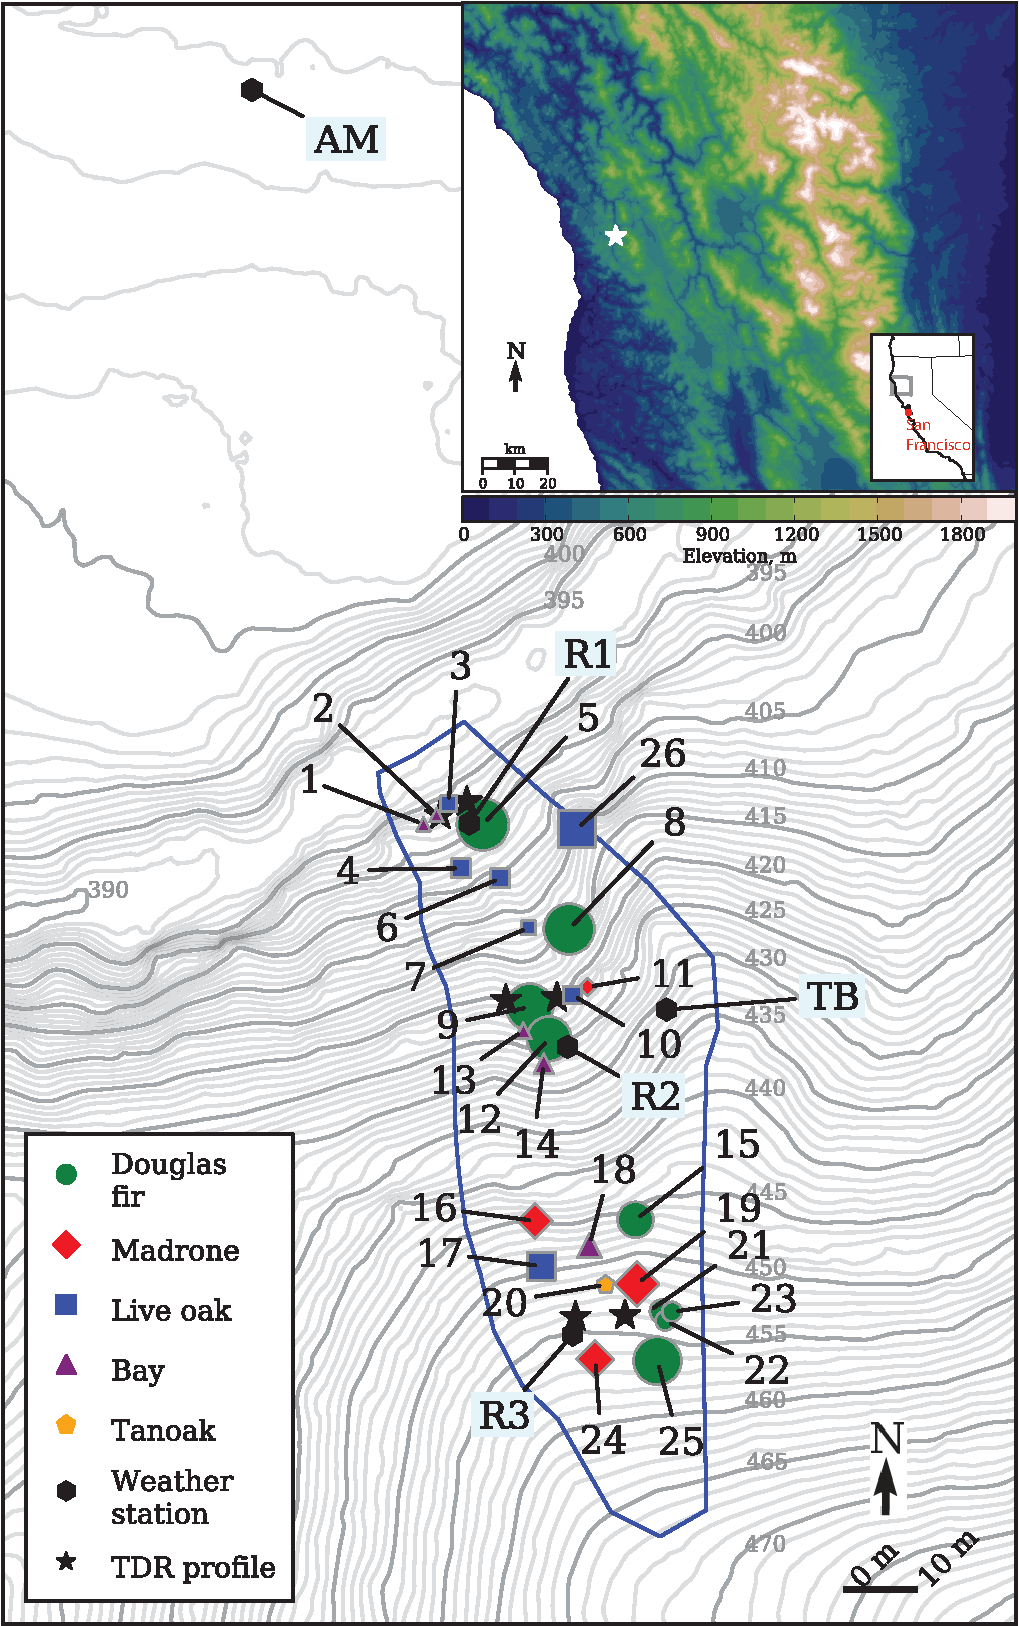
\includegraphics[width=0.9\textwidth]{ch1-sapflow/figures/Figure01.pdf}
\caption{Site map, showing topography, weather stations (R1, R2, R3, TB, AM), TDR profiles, and trees instrumented with sap flow sensors.  Symbols for instrumented trees are scaled by the tree diameter.  Tree numbers correspond with those in Table \ref{tbl:tree_props}.  Light gray numbers show elevation above sea level, in m.  Large inset: regional topography near the Angelo Coast Range Reserve (white star) [\textit{GLOBE Task Team et al.}, 1999 XXXX].  Small inset: California, with gray box outlining the region displayed in the large inset, and red dot showing San Francisco.}
\label{fig:sapflow_map}
\end{figure}

The study site (39.729$^{\circ}$N, 123.644$^{\circ}$W) is located in the University of California Angelo Coast Range Reserve (ACRR) in Mendocino County, northern California, about 260 km north of San Francisco (Figure \ref{fig:sapflow_map} inset).  The ACRR sits in the Eel River watershed about 16 km east of the Pacific coast, just outside the coastal fog belt in the complex topography of the California Coast Range. The highest point in the ACRR, Cahto Peak, has an elevation of 1300 m above sea level, and the base elevation of the reserve is 400 m above sea level.
	
The field site, known as ``Rivendell'', is a small (4000 m$^2$), north-facing hillslope that drains to Elder Creek, a tributary of the South Fork Eel River (Figure \ref{fig:sapflow_map}).  Rivendell is the subject of an interdisciplinary collaborative project to study the lifecycle of water through a steep hillslope, and over 700 separate instruments have collected over 100 million data points between 2007 and May 2012.  The site has an average slope of approximately 32 degrees.  The subsurface structure consists of a thin soil mantle over a layer of highly fractured sedimentary rock, underlain by unweathered bedrock with very low permeability.  The fractured, weathered bedrock zone transitions with depth from relatively soil-like granular material to low-permeability bedrock bounded by fractures.  Both the soil mantle and the weathered rock layer are thicker at the hill crest (60 cm soil and 20 m weathered rock) and thinner at the base of the hill (0-30 cm soil and 5 m weathered rock) [\cite{rempe2010}].

The old-growth forest in the ACRR consists primarily of Douglas-fir (\textit{Pseudotsuga menziesii}), coast redwood (\textit{Sequoia sempervirens}), interior live oak (\textit{Quercus wislizeni}), tanoak (\textit{Notholithocarpus densiflorus}), Pacific madrone (\textit{Arbutus menziesii}), and California bay (\textit{Umbellularia californica}).  In the Eel River watershed, Douglas-fir constitutes approximately 40\% of tree basal area [XXXX \textit{Woudenberg et al.}, 2010] and is commonly associated with Pacific madrone, tanoak, live oak, and other species in the Pacific Douglas-fir alliance in coastal northern California [XXXX r\textit{USDA}, 2005].  At the study site, Douglas-firs form the overstorey, with heights up to 55-60 m, while live oaks, bays, Pacific madrones, and tanoaks form the lower canopy, reaching heights of approximately 20 m.  Below the lower canopy, there are smaller (5-10 m) trees of all species. There is no dense ground cover. Douglas-firs, live oaks, tanoaks, and bays are evenly distributed across the hillslope, while Pacific madrones occur more frequently upslope.  Douglas-fir is a needleleaf tree, while live oaks, tanoaks, Pacific madrones, and bays are broadleaf trees, but all of these species are evergreen. The rooting depths of trees at this site have not been determined, but during drilling of wells at the site, roots of unidentified species were observed most densely in the top several meters and with decreasing density to a depth of 15.2 m.

Climatic variables, including air temperature (\textit{T}, $^{\circ}$C), relative humidity (\textit{RH}, \%), solar radiation (\textit{I}, W/m$^2$), and precipitation (\textit{P}, mm), are measured at five weather stations at the site (Figure \ref{fig:sapflow_map}).  One weather station (TB) is located approximately 30 m above ground in the tree canopy, three weather stations (R1, R2, and R3) are located 1 m above the ground in an along-slope transect, and one weather station (AM) is located in an open meadow with full clearance, across the stream from the site.  The weather stations on the site (TB, R1, R2, and R3) are used here to characterize the \textit{VPD} at the site (\textit{T} and \textit{RH} from Vaisala HMP45C-L sensors at R1, R2, R3, and from a Vaisala WXT510 sensor at TB; Vaisala, Helsinki, Finland), while the meadow weather station (AM) is used for unobstructed \textit{I} and gross \textit{P} (Li-Cor LI200X-L pyranometer, Li-Cor, Lincoln, NE, USA; and Campbell Scientific TE525 tipping bucket rain gauge, Campbell Scientific, Logan, UT, USA).  All meteorological and soil moisture measurements were recorded with CR1000 dataloggers (Campbell Scientific) at intervals of 15 minutes until 2010 and 5 minutes beginning in 2010, and transmitted wirelessly and automatically to an online server; the entire system is powered only by solar cells.

Both shallow soil moisture and groundwater level are measured at Rivendell.  Depth profiles of $\theta$ (with a sensor placed every 5 to 10 cm down to a depth of 50 to 70 cm) are measured continuously with time domain reflectometer sensors (TDR; TDR100, Campbell Scientific) at six locations on the hillslope (Figure \ref{fig:sapflow_map}).  The TDR sensors are 7.5 cm long and are located in \textit{in situ} material: small trenches were dug in order to insert the probes horizontally into the soil or soil-like material in rock fractures, after which the trenches were backfilled with excavated material.  Measured dielectric values are converted to volumetric $\theta$ (m$^3$ water/m$^3$ total) using the standard Topp equation [\cite{topp1980electromagnetic}].  Groundwater level is monitored at 12 on-site wells.

Volumetric $\theta$ measurements are filtered to exclude values outside the sensor's valid range and averaged over each day to reduce noise (no diurnal cycle is evident at this site, in contrast to other Douglas-fir sites [\cite{brooks2006}; \cite{Warren:2007ly}]).  The daily-average values are then averaged across all depths for each profile; each profile average is normalized by its maximum to convert to relative $\theta$ (\%); and the six profiles on the slope are then averaged to produce a site-averaged $\theta$ time series.  The conversion to relative soil moisture is performed because no site-specific TDR calibration was performed.  We explain our reasoning for the site averaging in the Discussion, Section \ref{sec:sapflow_soilmoisture}.

\subsection{Sap flow measurement}
Sap velocity, the velocity of water through the xylem parallel to the axis of the tree trunk, is measured in 26 trees using 39 heat ratio method sensors (ICT International, Armidale, Australia; \cite{burgess2001improved}) installed 1 m above the ground in the tree trunks.  The tree locations, species, and diameters at breast height are shown in Figure \ref{fig:sapflow_map}, with the symbol size scaled by tree diameter, and the properties of each sensor are listed in Table \ref{tbl:tree_props}.  The trees were chosen to represent the distribution of tree species and sizes on the hillslope, within the constraints of accessibility on the steep slope and a limited number of sensors.  Multiple trees were instrumented for each species except tanoak (1 tree), which was sparse on this hillslope (uncharacteristically for this region.)  Before installing the sensors, bark was removed to the cambium from an approximately 5 cm x 5 cm area.  Each sensor measures the velocity of a heat pulse emitted by the sensor at two radial depths in the xylem: 12.5 mm and 27.5 mm.  These depths are not precise because of minor errors in sensor placement; errors in probe spacing are corrected using the procedure in \cite{burgess2001improved}.  For this procedure, we assume zero flow at times when water stress is expected to be minimal: pre-dawn (within 3 hours before sunrise), high relative humidity (between 92 and 95\%), no solar radiation, no daily rain, and between January and March.  Sensors were moved in late 2010 to minimize wounding, creating two stages of deployment (2009-2010, and 2011.)  Because we did not measure wound diameters around the probes (as that would be destructive), we assume a wound diameter of 0.2 mm (a central value from Table 1 in \cite{burgess2001improved}) for all sensors; the wound correction is a linear factor and is thus removed by the normalization described below (Section \ref{sec:normalization}).  Heat pulse velocity was recorded on ICT SL5 Smart Loggers (ICT International, Armidale, Australia) at 30-minute intervals.

\begin{table}
  \caption{Sap flow sensor properties, including tree, sensor ID, stage of deployment, species, DBH (diameter at breast height), nearest weather station, active depth (radial sensor position with larger sap velocity), 99.5th percentile instantaneous sap velocity for each sensor position, 12.5 mm - 27.5 mm sensor correlation ($R^2$ coefficient comparing velocities at the two measured radial positions), 99.5th percentile daily integral sap velocity for the active sensor depth, lag time of sap velocity relative to radiation, lag time of sap velocity relative to VPD, wood dry density at the two sensor positions, and wood water content at the two sensor positions.}
  \label{tbl:tree_props}
  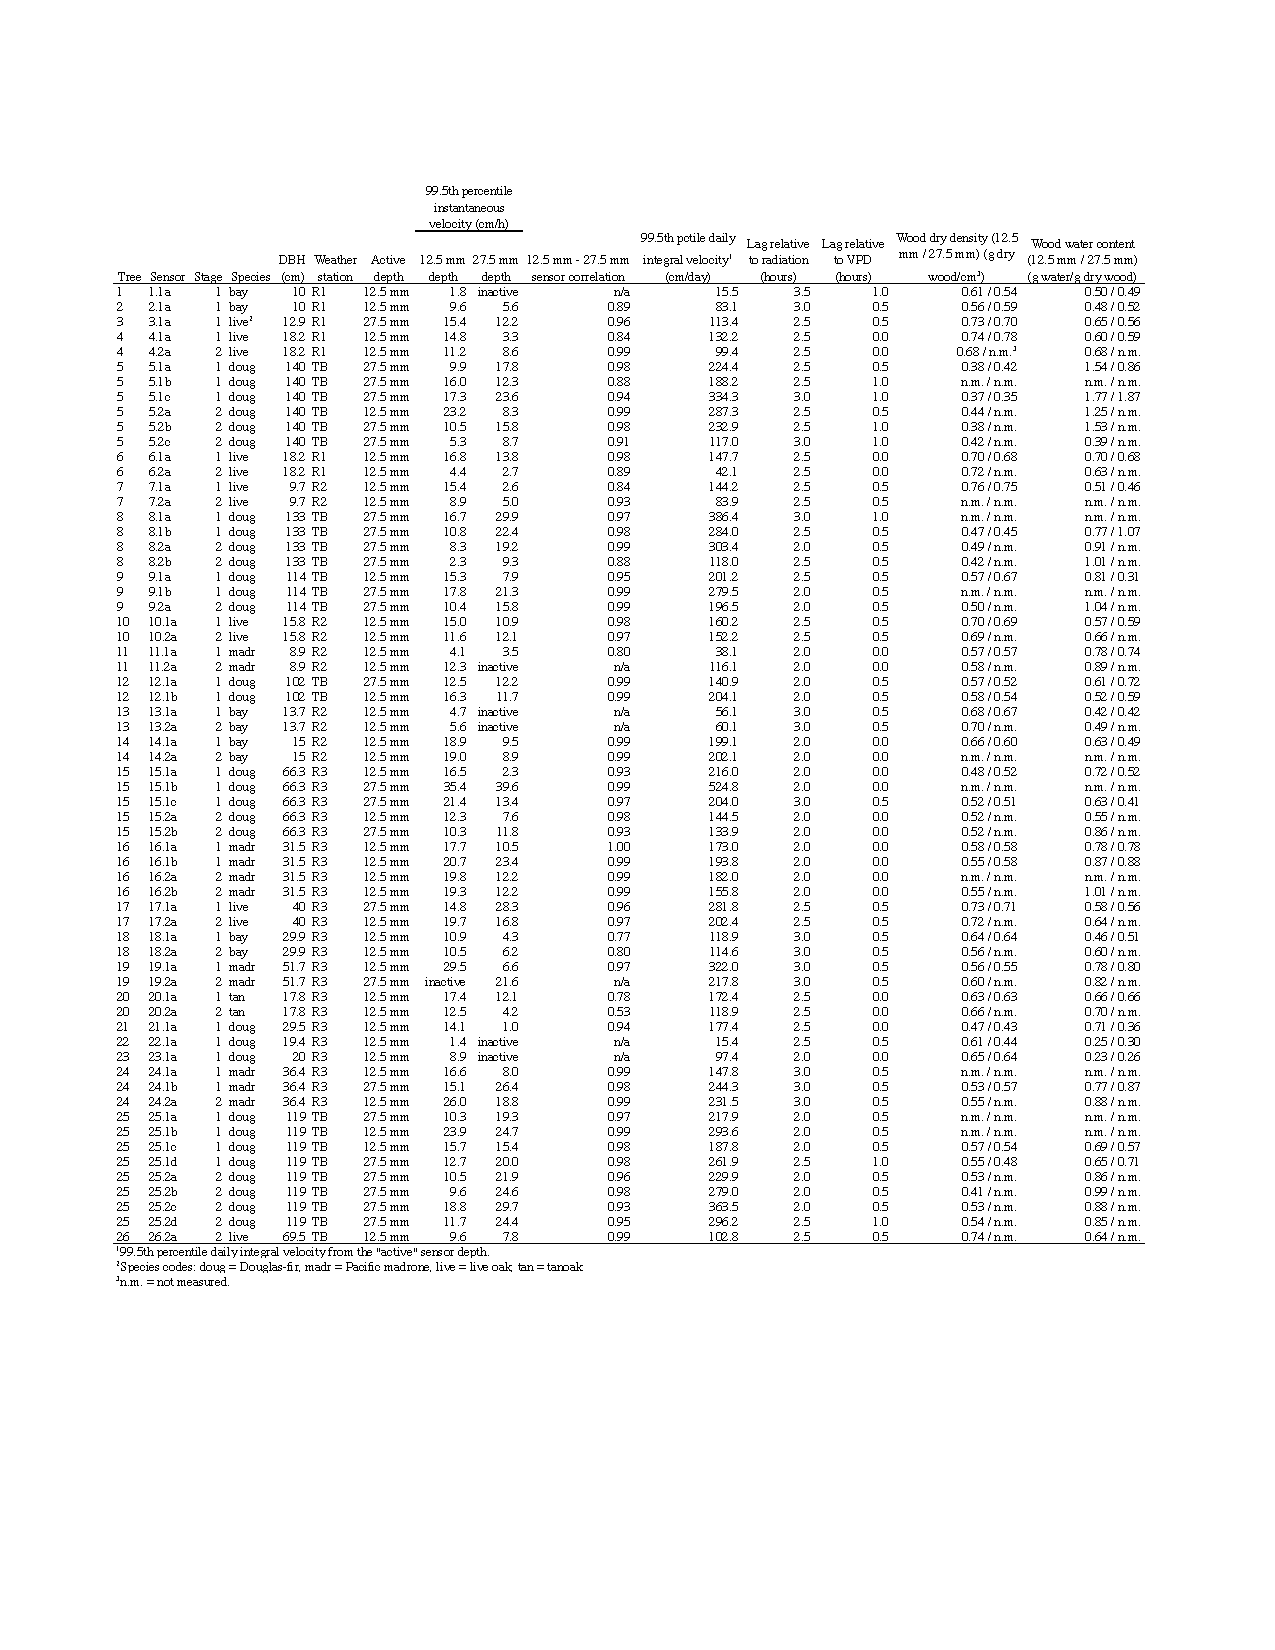
\includegraphics[width=\linewidth]{ch1-sapflow/tables/Table1.pdf}
\end{table}

Wood density and water content were measured by taking cores with an increment borer in October 2010 and October 2012, and these properties are used to convert heat pulse velocity to sap velocity [\cite{burgess2001improved}].  For several sensors, wood density and water content were not measured (Table \ref{tbl:tree_props}); for these sensors, the species-averaged values were used.  Because water content was only measured once at the end of each stage, we used a constant value throughout the year.  Uncertainties associated with this assumption are discussed in Section \ref{sec:sapflow_soilmoisture}.

For the following analyses, for each sensor, the depth with the larger magnitude of velocity (i.e. the most ``active'' depth) is chosen.  Sap velocity is known to vary radially through the sapwood [\cite{cohen1985determination}; \cite{vcermak1992radial}; \cite{nadezhdina2002radial}; \cite{ford2004assessing}]; in our measurements, the velocities at 12.5 mm and 27.5 mm differed in magnitude but were highly correlated for almost all sensors ($R^2$ values listed in Table \ref{tbl:tree_props}); as such, we include only one depth per sensor in order to avoid redundancy.

Finally, we add the caveat that we treat sap velocity as proportional to transpiration.  We discuss this assumption in Section \ref{sec:sapflow_soilmoisture}.

\subsection{Normalization}
\label{sec:normalization}
For most of our analyses, we use normalized sap velocities.  Normalizing allows us to compare temporal dynamics and environmental responses between sensors with very different absolute magnitudes, and eliminates the time-invariant differences in absolute velocity due to azimuthal, radial, or between-tree variation in wood properties.  We employ normalization on two time scales.   The first normalizes instantaneous (30-minute frequency) measurements by dividing by the 99.5th percentile value of that sensor (to avoid normalizing by an outlier); this normalization is used for analyzing responses to environmental drivers (Sections \ref{sec:mcmc} and \ref{sec:envresponse}).  In the second, daily integrals of sap velocity are normalized by dividing by the 99.5th percentile daily integral for each sensor; the normalized daily integrals are used for analyzing seasonal dynamics (Sections \ref{sec:pca} and \ref{sec:seasonal}), since the diurnal cycle is removed.  Sensors are normalized separately for each stage of deployment, because azimuthal variations in wood properties caused differences in absolute magnitude of velocity when sensors were moved within a tree.

\subsection{Principal Component Analysis}
\label{sec:pca}
We use principal component analysis (PCA) to find the dominant spatial and, importantly, temporal sap flow patterns in the sap flow dataset, and to compare the dominant seasonality patterns between trees, across space and between species.  PCA, also known as empirical orthogonal function analysis [\cite{lorenz1956empirical}], reduces a dataset with many points in space and time to a few orthogonal patterns that explain most of the variance. These orthogonal patterns are determined empirically from the data, as the eigenvectors of the covariance matrix.  PCA yields a series of temporal functions (PCs), with a corresponding series station weighting factors (EOFs), which represent how strongly each time function (PC) contributes to the actual time series at a given station.  The pairs of time-space functions (PC$_m$ and EOF$_m$) are ordered by the fraction of the total dataset variance that each explains.

We perform PCA separately on each of the two stages of sensor deployment (2009-2010, and 2011), because many of the time series were discontinuous across the sensor move; many sensors failed after the move or were placed in roots, which were not analyzed in the present study.  In order to maximize the amount of data included in the analysis, we performed PCA on the two stages separately.  Performing PCA on the two stages also has the advantage of providing replication of the dominant patterns of variability; similarity between results from the two stages would indicate interannual robustness of the seasonal patterns.

Days with missing data are excluded.  The analyses are performed on normalized daily integral values, subtracting each sensor's mean for the analysis period to focus on the temporal variability. The analysis is performed in Python, using the NumPy linalg function \textit{eig}. In the following, we focus on the first two PC-EOF pairs for each analysis, as they together explain over 90\% of the variance.

\subsection{MCMC estimation of environmental response parameters}
\label{sec:mcmc}
We quantify the relationship between each sensor's instantaneous sap flow and environmental drivers using the Jarvis model [\cite{jarvis1976interpretation}], which parameterizes stomatal conductance in terms of empirical functions of \textit{VPD}, \textit{I}, and $\theta$.

We begin with the assumption that each sensor's instantaneous normalized sap velocity ($v_n$, unitless) is proportional to the tree's transpiration ($E$, liters/day), scaled by a multiplier, $\alpha$ (liters/day), the product of maximum sap velocity, sap wood cross-sectional area, and the profile of sap velocity as a function of radius:

\begin{equation} % equation 1
\label{eqn:sf1}
E = \alpha \cdot v_n.
\end{equation}

Transpiration also equals the product of the tree's bulk canopy conductance ($g_c$, liters/day/kPa) and the leaf-to-air vapor pressure difference (which we approximate with the air \textit{VPD}.)  Thus,

\begin{equation} % equation 2
E = g_c \cdot VPD.
\end{equation}

Following the Jarvis model, canopy conductance ($g_c$) is modeled as a maximum conductance ($g_{cmax}$, liters/day/kPa), reduced by empirical multiplicative functions, ranging from 0 to 1, of important environmental modifiers: \textit{VPD}, $\theta$, and $I$ [\cite{jarvis1976interpretation}; \cite{oren1999survey}; \cite{waring2011generalizing}].

\begin{equation}  % equation 3
g_c = g_{cmax} \cdot f_{VPD}(VPD) \cdot f_{\theta}(\theta) \cdot f_I(I).
\end{equation}

The functions of environmental modifiers are analytical parameterizations based on previous empirical observations.  For the atmospheric evaporative demand function, $f(VPD)$, we use an asymptotic function [\cite{lohammar1980fast}; \cite{lindroth1986numerical}; \cite{dang1997regulation}],

\begin{equation}  % equation 4
f_{VPD}(VPD) = \frac{1}{1+VPD/D_o},
\end{equation}
where $D_o$ (kPa) describes the sensitivity of $g_c$ to \textit{VPD}.

The water supply function, $f(\theta)$, is modeled as a sigmoid function, chosen because it is a continuous function that represents the threshold limitation of transpiration by $\theta$ in very dry soils; this is a continuous functional form that approximates the piecewise-linear Feddes model [\cite{feddes}; \cite{chen2008observations}]:

\begin{equation}  % equation 5
f_{\theta}(\theta) = \frac{1}{1+\exp(-\beta(\theta-\theta_o))},
\end{equation}
where $\beta$ (unitless) measures the rate of decrease of transpiration at low $\theta$, and $\theta_o$ (unitless) is the value of $\theta$ at which the transpiration decline is centered.  These parameters can be related to the more standard stress point and wilting point of the Feddes model by estimating the $\theta$ at which the sigmoid function begins to decline (the stress point) and the $\theta$ at which the sigmoid function is approximately zero (the wilting point.)

The radiation function, $f(I)$, is modeled as a linear function, after \cite{waring2011generalizing}:

\begin{equation}  % equation 6
f_I(I) = \gamma \cdot (I-1000 \, {\rm W/m^2})+1,
\end{equation}
where $\gamma$ ((W/m$^2$)$^{-1}$) is the sensitivity of transpiration to \textit{I}, and $f(I)$ is prescribed to be maximum (equal to 1) at maximum \textit{I} (1000 W/m$^2$).

Thus, we model normalized sap velocity as a function of \textit{VPD}, $\theta$, \textit{I}, and five parameters (considering $g_{cmax}/\alpha$ (kPa$^{-1}$) as a single parameter):

% equation 7
\begin{align}
\label{eqn:sapflow_jarvis}
v_n & =  \frac{g_{cmax}}{\alpha} \cdot VPD \cdot f_{VPD}(VPD) \cdot f_{\theta}(\theta) \cdot f_I(I) \nonumber \\ 
& =  \frac{g_{cmax}}{\alpha} \cdot \frac{VPD}{1+\frac{VPD}{D_o}} \cdot \frac{1}{1+\exp(-\beta(\theta-\theta_o))} \cdot (\gamma \cdot (I-1000)+1).
\end{align}

We estimate these five parameters for each sensor using a Markov chain Monte Carlo (MCMC) method, described in the appendix (Section \ref{sec:sapflow_appendix}).  The MCMC method allows us to quantify uncertainty in the parameters and avoid local minima traps on the complex $\chi ^2$ surface that might hinder optimization algorithms.  Each sap flow sensor is matched with the nearest weather station: the canopy weather station (TB) is used for the overstorey trees, while the nearest ground station (R1, R2, or R3) is used for the understorey canopy trees, including small Douglas-firs.  Incoming \textit{I} measured in the open meadow (station AM, Figure \ref{fig:sapflow_map}) is used for all sensors, because \textit{I} was only measured at station AM.  \textit{VPD}, \textit{I}, and $\theta$ were subsampled to the 30-minute frequency of sap flow measurements.  For each tree, sap velocity is lagged relative to \textit{I} and \textit{VPD} by a lag time determined by the maximum lag correlation for that tree's average timeseries, similar to the procedure in \cite{dragoni2009decoupling}; lag times are listed in Table \ref{tbl:tree_props}.  The analysis is performed using times when \textit{I} was greater than zero (i.e., daytime observations) and \textit{VPD} was greater than 0.1 kPa.  Days with more than 2 mm of rain were excluded, because on those days leaves were probably covered with water and sap velocity thus was probably not controlled by stomatal response to the environment.  The site-averaged, daily-averaged $\theta$ is used for all sensors, as described in Section \ref{sec:sapflow_sitedesc}.  Parameters are also estimated for each species as a whole, using the average $v_n$ at each measurement from all sensors from a given species; these are referred to as the ``species-averaged timeseries" parameters.

\subsection{Estimates of regional transpiration}
\label{sec:sapflow_regmeth}
We use the species-averaged timeseries of normalized sap velocity, along with Forest Inventory and Analysis (FIA) [XXXX \textit{Woudenberg et al.}, 2010] observations of tree size and species distributions in the Eel River watershed, to estimate the contribution of each species to regional transpiration.  We estimate regional transpiration, rather than hillslope transpiration at our particular site, because regional distributions of trees by species and diameter are available from the FIA inventory, but no species-diameter inventory has been conducted at our particular site.  This scale jump requires simplifications and assumptions (described below), and as such, our calculations are a rough best estimate and an attempt to bound the range of possible forest transpiration in this region from a bottom-up perspective.  

Transpiration was estimated using Equation \ref{eqn:sf1}, with $v_n$ calculated using the species-averaged timeseries Jarvis parameters, and $\alpha$ disaggregated as follows.  Transpiration for a single tree ($E_{tree}$, cm m$^2$/hr) is

% equation 8
\begin{align}
E_{tree} & = \int_{r_{inner}}^{r_{outer}} 2\pi r \, v(r) \, \mathrm{d}r \nonumber \\ 
& =  \int_{r_{inner}}^{r_{outer}}  2\pi r \, v_{max} \, v_{n} \, f_{prof}(r) \, \mathrm{d}r,
\end{align}
where $r$ is radial position on a cross-section of the tree, $r_{inner}$ is the radial position of the sapwood-heartwood boundary (meters), $r_{outer}$ is the radial position of the sapwood-bark boundary (meters, here treated as approximately equal to half the tree diameter at breast height, $d/2$), $v(r)$ is the sap velocity as a function of radial position in the sapwood (cm/hr), and $f_{prof}(r)$ is a linear function between 0 and 1 describing the radial profile of sap velocity relative to the velocity at the outer edge (described below).  In this equation, $v_n$ and $v_{max}$ can be pulled out of the integral, and the resulting term $2\pi \, v_{max} \, \int_{r_{inner}}^{r_{outer}}  r \, f_{prof}(r) \, \mathrm{d}r$ is equal to $\alpha$ in Equation \ref{eqn:sf1}.

The thickness of the sapwood is estimated using two site-specific sapwood thickness--diameter relations, derived from 21 tree cores taken near Rivendell (15 Douglas-fir samples ($R^2=0.88$) and 6 Pacific madrone samples ($R^2=0.83$)):
\begin{align}
\label{eqn:sapwood}
w_{sap,Douglas-fir} = 0.12d+0.0089\\
w_{sap,madrone} = 0.1d+0.0071 ,
\end{align}
and
\begin{equation}
r_{inner} = d/2-w_{sap},
\end{equation}
where $w_{sap}$ is sapwood thickness (m).  Our Douglas-fir relationship is roughly similar to the one found by \cite{smith1966variation} for Douglas-fir.  

In addition, for other broadleaf species, we use the ring-porous equation from \cite{wullschleger2001transpiration}:
\begin{equation}
\label{eqn:sapwood2}
r_{inner,Wullschleger} = \sqrt{\left(\frac{d}{2}\right)^2-\frac{1.637d^{0.56}}{\pi}}.
\end{equation}
This equation is used for non-Pacific-madrone broadleaf species.

Sap velocity was approximated as a linear function of radial position in the sapwood, based on observations that sap velocity is often lower in the inner sapwood than in the outer sapwood [\cite{ford2004assessing}; \cite{cohen1985determination}; \cite{vcermak1992radial}; \cite{nadezhdina2002radial}].  The velocity at the outer edge of the sapwood was estimated as the product of a time-invariant maximum velocity ($v_{max}$, cm/hr) and a time-varying normalized velocity ($v_n$, unitless), approximated as the species-averaged timeseries of measured normalized sap velocity.  $v_{max}$ values for each species were treated as independent of tree diameter and were approximated with the species-averaged maximum instantaneous velocities from Table \ref{tbl:sapflow_maxvel}.  Sap velocity is assumed to be independent of azimuth, or equivalently, we assume that $v_{max,sp}$ is an average of the maximum velocity around the bole of a tree.

\begin{table}
  \caption{Species-averaged maximum sap velocities.}
  \label{tbl:sapflow_maxvel}
  \begin{tabular}{l r}
  \hline
  Species & Velocity (cm/h) \\
  \hline
  Douglas-fir & 18.2 \\
  Pacific madrone & 19.5 \\
  live oak & 14.0 \\
  bay & 10.1 \\
  tanoak & 15.0 \\
  \hline
  \end{tabular}
\end{table}

Because the radial profile of sap velocity is not well constrained with our measurements, we test three possible velocity profiles, with $v(r) = v_{max} \, v_n \, f_{prof}(r)$: (1) constant velocity across the sapwood ($f_{prof}(r) = 1$); (2) velocity decreasing linearly from $v_{max} \, v_n$ at the outer edge of the sapwood to $0.5 \, v_{max} \, v_n$ at the inner edge of the sapwood ($f_{prof}(r) = 1+\tfrac{0.5}{w_{sap}}(r-r_{outer})$ ); and (3) velocity decreasing linearly from $v_{max} \, v_n$ at the outer edge of the sapwood to 0 at the inner edge of the sapwood ($f_{prof}(r) = 1+\tfrac{1}{w_{sap}}(r-r_{outer})$ ).

Transpiration is scaled from a single tree to the regional scale using distributions of tree species and sizes measured in the Eel River watershed by the FIA program, binned by diameter in 5 cm bins [\textit{Woudenberg et al.}, 2010] (locations of FIA plots are intentionally ``fuzzed and swapped'' for privacy reasons, but the provided coordinates are ``similar'' to the true coordinates with an unspecified offset).  The FIA surveyed 321 forested plots within the Eel Watershed.  Figure \ref{fig:sapflow_abundances} shows $N_{i,sp}$, the number of trees per km$^2$ in each diameter bin ($i$) for major species categories in the watershed ($sp$), averaged over the 321 FIA plots.

\begin{figure}[here]
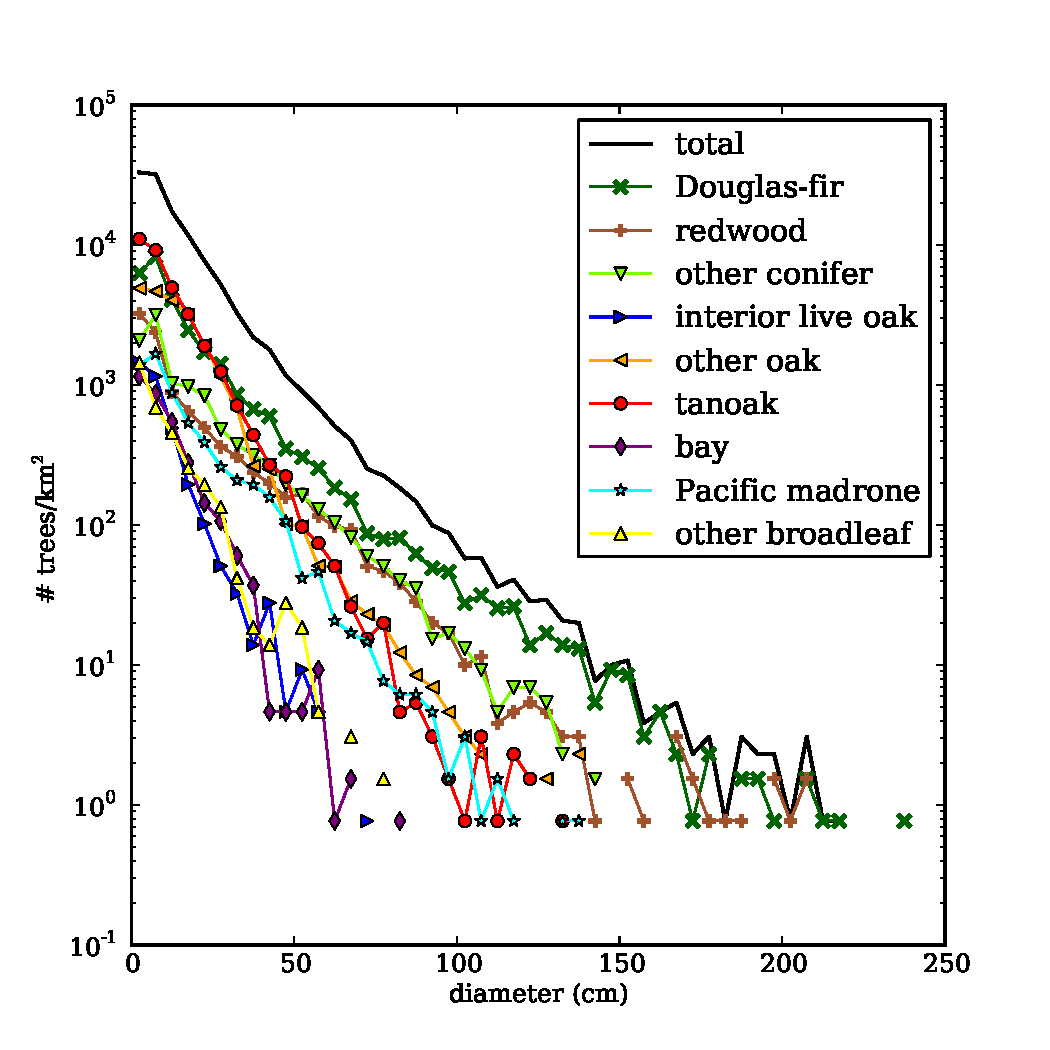
\includegraphics[width=0.9\textwidth]{ch1-sapflow/figures/Figure02.pdf}
\caption{Counts of trees per km$^2$ in major species categories, binned diameter; from FIA plots in the Eel River watershed [\textit{Woudenberg et al.}, 2010 XXXX].  The category ``other conifer'' includes knobcone pine, Jeffrey pine, sugar pine, Western white pine, bishop pine, ponderosa pine, California foothill pine, white fir, grand fir, red fir, Pacific yew, western hemlock, incense cedar, and Sitka spruce.  The category ``other oak'' includes California live oak, canyon live oak, blue oak, Oregon white oak, California black oak, and California white oak.  The category ``other broadleaf'' includes bigleaf maple, California buckeye, red alder, white alder, giant chinkapin, and bitter cherry.}
\label{fig:sapflow_abundances}
\end{figure}

Regional transpiration due to each species (mm/d) is then estimated by summing individual tree transpiration of the species over all diameter bins ($i$):
\begin{align}
\label{eqn:transpreg}
T_{sp} &= \sum_{i} N_{i,sp} \, E_{tree,i,sp} \nonumber \\
&= 2\pi \, v_{max,sp} \, v_{n,sp} \, \sum_{i} N_{i,sp} \, \int_{r_{inner,i}}^{r_{outer,i}}  r \, f(r) \, \mathrm{d}r ,
\end{align}
and subsequently applying a unit conversion factor of $(10 \tfrac{mm}{cm}) (24 \tfrac{hr}{day}) (10^{-6} \tfrac{km^2}{m^2})$.  Total regional transpiration is estimated by summing transpiration estimated for all species, using the averaged time series of measured species to represent unmeasured but similar species.  All conifers, including redwoods, are assigned the Douglas-fir time series; all oaks, both evergreen and deciduous, are assigned the interior live oak time series; and all other unmeasured broadleaf trees are assigned the Pacific madrone time series, in order to give an upper-bound estimate on dry season transpiration.  Thus, we effectively bin species into categories of needleleaf evergreen and broadleaf evergreen; these assumptions are necessary because redwoods and major pine species were not measured due to their scarcity at our site.  In addition, we calculate regional transpiration in two extreme hypothetical cases, using the FIA total tree size distribution (black line in Figure \ref{fig:sapflow_abundances}): one case in which all trees are assigned the Douglas-fir time series, and another case in which all trees are assigned the Pacific madrone time series. 

The sap-flow-based regional transpiration estimates are compared with remotely-sensed MODIS-derived estimates of ET [XXXX \textit{Mu et al.}, 2007.]  The MODIS algorithm uses remotely-sensed LAI and modeled stomatal response based on an assigned plant functional type (which for this region is evergreen needleleaf forest), combined with meteorology from atmospheric reanalysis, to estimate stomatal conductance and ET.  No soil moisture or subsurface information is explicitly included.  Two spatial scales of the MODIS-derived estimate are presented: the 1 km x 1 km pixel nearest to Rivendell (pixel centered about 450 m east of Rivendell), and the average for all pixels in the Eel River watershed.  Our goals in comparing our estimated to the MODIS-derived estimate are a) to confirm that our estimates are the right order of magnitude, and b) to compare the seasonal timing of transpiration between the methods.

